\documentclass[11pt,a4paper]{report}%especifica o tipo de documento que tenciona escrever: carta, artigo, relatório... neste caso é um relatório
% [11pt,a4paper] Define o tamanho principal das letras do documento. caso não especifique uma delas, é assumido 10pt
% a4paper -- Define o tamanho do papel.

\usepackage[portuges]{babel}%Babel -- irá activar automaticamente as regras apropriadas de hifenização para a língua todo o
                                   %-- o texto gerado é automaticamente traduzido para Português.
                                   %  Por exemplo, “chapter” irá passar a “capítulo”, “table of contents” a “conteúdo”.
                                   % portuges -- específica para o Português.
\usepackage[utf8]{inputenc} % define o encoding usado texto fonte (input)--usual "utf8" ou "latin1

\usepackage{graphicx} %permite incluir graficos, tabelas, figuras
\usepackage{url} % para utilizar o comando \url{}
\usepackage{enumerate} %permite escolher, nas listas enumeradas, se os iems sao marcados com letras ou numeros-romanos em vez de numeracao normal

%\usepackage{apalike} % gerar biliografia no estilo 'named' (apalike)

\usepackage{color} % Para escrever em cores
\usepackage{float}
\usepackage{tabto}

\usepackage{multirow} %tabelas com multilinhas
\usepackage{array} %formatação especial de tabelas em array

\usepackage[pdftex]{hyperref} % transformar as referências internas do seu documento em hiper-ligações.

%Exemplos de fontes -- nao e vulgar mudar o tipo de fonte
%\usepackage{tgbonum} % Fonte de letra: TEX Gyre Bonum
%\usepackage{lmodern} % Fonte de letra: Latin Modern Sans Serif
%\usepackage{helvet}  % Fonte de letra: Helvetica
%\usepackage{charter} % Fonte de letra:Charter

\definecolor{saddlebrown}{rgb}{0.55, 0.27, 0.07} % para definir uma nova cor, neste caso 'saddlebrown'

\usepackage{listings}  % para utilizar blocos de texto verbatim no estilo 'listings'
%paramerização mais vulgar dos blocos LISTING - GENERAL
\lstset{
	basicstyle=\small, %o tamanho das fontes que são usadas para o código
	numbers=left, % onde colocar a numeração da linha
	numberstyle=\tiny, %o tamanho das fontes que são usadas para a numeração da linha
	numbersep=5pt, %distancia entre a numeração da linha e o codigo
	breaklines=true, %define quebra automática de linha
    frame=tB,  % caixa a volta do codigo
	mathescape=true, %habilita o modo matemático
	escapeinside={(*@}{@*)} % se escrever isto  aceita tudo o que esta dentro das marcas e nao altera
}
%
%\lstset{ %
%	language=Java,							% choose the language of the code
%	basicstyle=\ttfamily\footnotesize,		% the size of the fonts that are used for the code
%	keywordstyle=\bfseries,					% set the keyword style
%	%numbers=left,							% where to put the line-numbers
%	numberstyle=\scriptsize,				% the size of the fonts that are used for the line-numbers
%	stepnumber=2,							% the step between two line-numbers. If it's 1 each line
%											% will be numbered
%	numbersep=5pt,							% how far the line-numbers are from the code
%	backgroundcolor=\color{white},			% choose the background color. You must add \usepackage{color}
%	showspaces=false,						% show spaces adding particular underscores
%	showstringspaces=false,					% underline spaces within strings
%	showtabs=false,							% show tabs within strings adding particular underscores
%	frame=none,								% adds a frame around the code
%	%abovecaptionskip=-.8em,
%	%belowcaptionskip=.7em,
%	tabsize=2,								% sets default tabsize to 2 spaces
%	captionpos=b,							% sets the caption-position to bottom
%	breaklines=true,						% sets automatic line breaking
%	breakatwhitespace=false,				% sets if automatic breaks should only happen at whitespace
%	title=\lstname,							% show the filename of files included with \lstinputlisting;
%											% also try caption instead of title
%	escapeinside={\%*}{*)},					% if you want to add a comment within your code
%	morekeywords={*,...}					% if you want to add more keywords to the set
%}

\usepackage{xspace} % deteta se a seguir a palavra tem uma palavra ou um sinal de pontuaçao se tiver uma palavra da espaço, se for um sinal de pontuaçao nao da espaço

\parindent=0pt %espaço a deixar para fazer a  indentação da primeira linha após um parágrafo
\parskip=2pt % espaço entre o parágrafo e o texto anterior

\setlength{\oddsidemargin}{-1cm} %espaço entre o texto e a margem
\setlength{\textwidth}{18cm} %Comprimento do texto na pagina
\setlength{\headsep}{-1cm} %espaço entre o texto e o cabeçalho
\setlength{\textheight}{23cm} %altura do texto na pagina

% comando '\def' usado para definir abreviatura (macros)
% o primeiro argumento é o nome do novo comando e o segundo entre chavetas é o texto original, ou sequência de controle, para que expande
\def\darius{\textsf{Darius}\xspace}
\def\antlr{\texttt{AnTLR}\xspace}
\def\pe{\emph{Publicação Eletrónica}\xspace}
\def\titulo#1{\section{#1}}    %no corpo do documento usa-se na forma '\titulo{MEU TITULO}'
\def\super#1{{\em Supervisor: #1}\\ }
\def\area#1{{\em \'{A}rea: #1}\\[0.2cm]}
\def\resumo{\underline{Resumo}:\\ }

%\input{LPgeneralDefintions} %permite ler de um ficheiro de texto externo mais definições

\title{\textbf{Trabalho Prático CG - 2022/2023}\\
       \textbf{Fase 1 - Primitivas Gráficas}\\ Licenciatura em Ciências da Computação\\ Universidade do Minho \\ Grupo 11
       } %Titulo do documento
%\title{Um Exemplo de Artigo em \LaTeX}
\author{Gonçalo Silva\\ (A95696) \and Nelson Almeida\\ (A95652) \and Nuno Costa\\ (A97610)
       } %autores do documento
\date{\today} %data

\begin{document} % corpo do documento

\begin{figure} %insere figuras
	
\includegraphics[width=0.4\textwidth]{images/logo.jpg}
\end{figure}

\maketitle % apresentar titulo, autor e data
\tableofcontents % Insere a tabela de indice
%\listoffigures % Insere a tabela de indice figuras
%\listoftables % Insere a tabela de indice tabelas

\chapter{Introdução} \label{chap:intro} %referência cruzada

Nesta primeira frase do trabalho prático da UC de Computação Gráfica, foi-nos proposto o desenvolvimento de dois programas, sendo eles o \emph{generator} e o \emph{engine}. O \emph{generator} tem a função de gerar um ficheiro com as informações do modelo requerido, isto é, criar um ficheiro com os vértices que constituem o modelo. Já o \emph{engine}, é responsável pela leitura de um ficheiro de configuração (escrito em XML) e pela exibição dos modelos obtidos nessa mesma leitura. De notar que este trabalho foi desenvolvido na liguagem de programação C++, juntamente com a API de computação gráfica \emph{OpenGL}.\\


\titulo{Um belo Projeto}
\area{Processamento de Linguagens}

Vamos agora indicar o conteúdo habitual da introdução de qualquer relatório.
\begin{description}  % Item com descrição
  \item[Enquadramento]  do tema proposto
  \item[Contexto] do tema que é abordado ao  longo do documento
  \item[Problema] o problema que se quer resolver e o objetivo do projeto relatado
  \item[Objetivo] do relatório
  \item[Resultados ou Contributos] -- pontos a evidenciar
  \item[Estrutura do documento] o que é abordado em cada capitulo.
\end{description}

Na Figura~\ref{fig:layoutDimensions} podemos ver o Layout dos Parâmetros do Formato de Página.

 \begin{figure} %insere figuras
       \centering % Coloca ao centro
       
\includegraphics[width=0.5\textwidth]{images/logo.jpg}
       % width=0.4\textwidth -- a figura é alterada de forma a que a largura seja 0.5 vezes a largura de um parágrafo normal (textwidth). A altura é calculada de forma a manter a relação altura/largura.
       \caption{Legenda da Figura} \label{fig:layoutDimensions} %legenda da figura
 \end{figure}

Letras gregas são estas $ \alpha \beta \gamma \delta $ que aqui demonstro EM FORMATO INLINE\\

Exemplo simples de fração múltipla \[ \frac{\frac{a * b + c}{4-3}}{3*5} \] simples  EM FORMATO
de DESTAQUE (nova linha)\\\\

Exemplo de LISTAS ENUMERADAS com LETRAS:
\begin{enumerate}[a)]
\item Listar todas as Pessoas identificadas, sem repetições;
\item Listar os Países e Cidades marcadas;
\item Listar as Organizações.\\ % mudar de linha
\end{enumerate}

Mais exemplos de LISTAS ENUMERADAS mas agora com NUMEROS e outras marcas:
\begin{enumerate}
\item Listar todas as Pessoas identificadas, sem repetições;
  \begin{enumerate}[i)]
     \item Listar todas as Pessoas identificadas, sem repetições;
     \item Listar os Países e Cidades marcadas;
     \item Listar as Organizações.\\ % mudar de linha
  \end{enumerate}
\item Listar os Países e Cidades marcadas;
  \begin{enumerate}[2.1)]
     \item Listar todas as Pessoas identificadas, sem repetições;
     \item Listar os Países e Cidades marcadas;
     \item Listar as Organizações.\\ % mudar de linha
  \end{enumerate}
\item Listar as Organizações.
    \begin{enumerate}[1)]
     \item Listar todas as Pessoas identificadas, sem repetições;
     \item Listar os Países e Cidades marcadas;
     \item Listar as Organizações.\\ % mudar de linha
  \end{enumerate}
\end{enumerate}

A mesma enumeração mas no standard DESCRITIVO:
\begin{description}
\item[Etape 1:] Listar todas as Pessoas identificadas, sem repetições;
\item[Etape 2:] Listar os Países e Cidades marcadas;
\item[Etape 3:] Listar as Organizações.\\\\
\end{description}


\textbf{Texto com cores}\\

\textcolor{blue}{texto em azul}\\
\textcolor{red}{texto em vermelho} \\
\textcolor{green}{texto em verde} \\
\textcolor{saddlebrown}{texto em Castanho} \\\\\\

\textbf{Texto destacado}\\

 \textbf{Texto NEGRITO} isto é um texto a NEGRITO \\%texto a negrito
 \textsf{Texto fonte SANS SERIF} isto é um texto SANS SERIF \\ % texto em fonte sans serif dentro de uma expressão matemática.
 \texttt{Texto fonte MÁQUINA}  isto é um texto fonte MÁQUINA\\ %texto na fonte de máquina de escrever dentro de uma expressão matemática.
 \textit{Texto a ITALICO} isto é um texto a ITALICO\\ %texto a italico
 \underline{Texto a SUBLINHADO} isto é um texto a SUBLINHADO \\\\ %texto a sublinhado

\textbf{Tamanhos de LETRA}\\

\large{largas -- large}\\
\Large{maiores -- Large}\\
\LARGE{muito grandes -- LARGE}\\
\huge{enormes --  huge}\\
\Huge{as maiores -- Huge}\\
\tiny{minúscula  -- tiny}\\
\scriptsize{muito pequena -- scriptsize} \\
\footnotesize{bastante pequena  -- footnotesize}\\
\small{pequena -- small}\\
\normalsize{normal -- normalsize}\\\\

\textbf{Exemplo de tabelas}\\
\begin{table}[h!] %Inserir tabela
\begin{center} %colocar a tabela ao centro
\begin{tabular}{ | c | c | c | } %desenha a tabela % {formato das colunas} -- 'l' a coluna e alinhada a esquerda;
                                                                              %'r' a coluna e alinhada a direita;
                                                                              %'c' a coluna e centralizada
  \hline  %desenhar uma linha horizontal de comprimento igual ao da tabela
  cell1 & cell2 & cell3 \\
  \hline
  cell4 & cell5 & cell6 \\
  cell7 & cell8 & cell9 \\
  \hline
\end{tabular}
\end{center}
\caption{Tabela Basica} \label{tab:tabelaBasica}
\end{table}


\begin{table}[h!] %Inserir tabela
\begin{center}
\begin{tabular}{ | m{5em} | p{1cm}| b{1in} | } % 'm': ao meio; 'b': em baixo; 'p': em cima
\hline
cell1 dummy text dummy text dummy text& cell2 & cell3 \\
\hline
cell5 & cell1 dummy text dummy text dummy text & cell6 \\
\hline
cell7 & cell8 & exemplo de uma linha muito extensa \\
\hline
\end{tabular}
\caption{Tabela em formato array } \label{tab:tabelaArray}
%Tabela em formato array é utilizada adaptar o comprimento da linha a largura da coluna
\end{center}
\end{table}


\begin{table}[h!]
\begin{center}
\begin{tabular}{ |l|c|r| }
\hline
col1 & col2 & col3 \\
  \hline
  \multirow{3}{4cm}{Multiple row} & cell2 & cell3 \\ %\multirow{num}{formato}{texto} - este comando faz concatenar num linhas em uma so
                                                    %parâmetro  {4cm} define um comprimento de '4cm' para a primeira coluna e centraliza o texto no meio da célula.

  & cell5 & cell6cell6 \\
  & cell8 & cell9cell9cell9 \\
  \hline
  cell4 & cell5 & cell6 \\
  \hline
\end{tabular}
\end{center}
\caption{Tabela com multilinhas}
\end{table}

\begin{table}[h!] %Inserir tabela
\begin{center}
\begin{tabular}{|l||c|c|c|c|c|}
\hline
\multicolumn{6}{|c|}{\textbf{Horário de Tópicos em Matemática - MAT}}\\
\hline
Horário    &Seg &Ter &Qua &Qui &Sex\\
\hline\hline
13:00-14:40&    &    &    &    & \\
\hline
14:55-16:35&    &    &    &    &TURMA N \\
\hline
16:35-18:15&TURMA N & &TURMA N & & \\
\hline
18:15-19:00& & & & & \\
\hline
\end{tabular}
\caption{Tabela com multicolunas}
\end{center}
\end{table}

\newpage

% colocar omitido um url de um site ou de um documento
Para mais informações sobre LATEX consultar o
 \href{http://www.ptep-online.com/ctan/lshort_port.pdf}{livro}.\\

%Colocar url de um site
 Para mais informações sobre LATEX
 consultar o livro\footnote{acessível em \url{http://www.ptep-online.com/ctan/lshort_port.pdf}}.


\chapter{Engine} \label{chap:engine} %capitulo e referencia cruzada
\section{Leitura do ficheiro de configuração} \label{sec:parsing} %seccao e referencia cruzada
Como sugerido, utilizou-se o \emph{tinyxml2} no auxílio à leitura do XML proveniente do ficheiro de configuração. O código do \emph{engine} possui duas funções responsáveis pela mesma, sendo elas:
\begin{enumerate}
\item void readXML(char* filename);
\item void readGroupXML(tinyxml2::XMLElement *group);
\end{enumerate}

De notar que a segunda função é apenas uma auxiliar da primeira função.

\section{Estruturação dos dados} \label{sec:structs}

\begin{figure}[H]
       \centering
       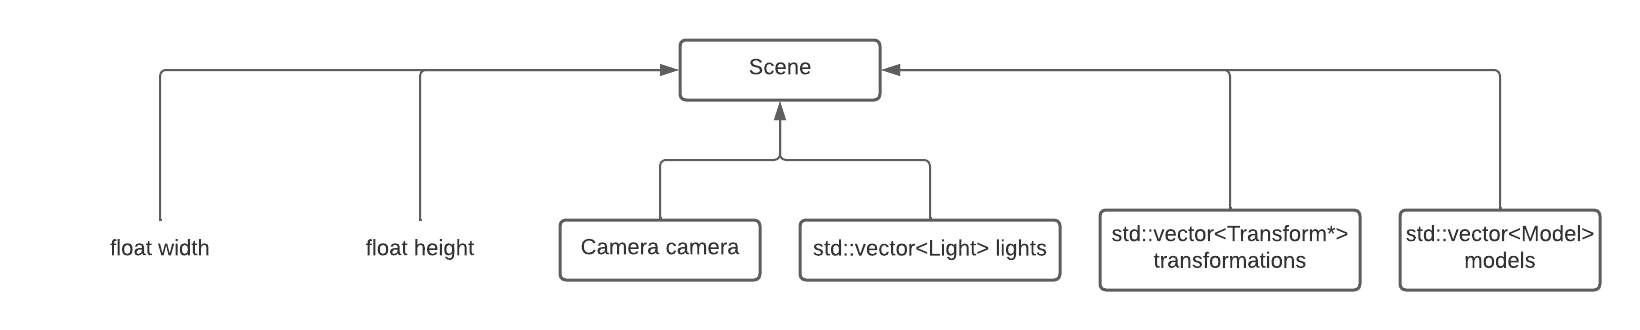
\includegraphics[width=0.9\textwidth]{images/data_structure_scene.png}
       \caption{Estrutura de dados \emph{Scene}} \label{fig:scene} 
\end{figure}
\begin{figure}[H]
	\centering
	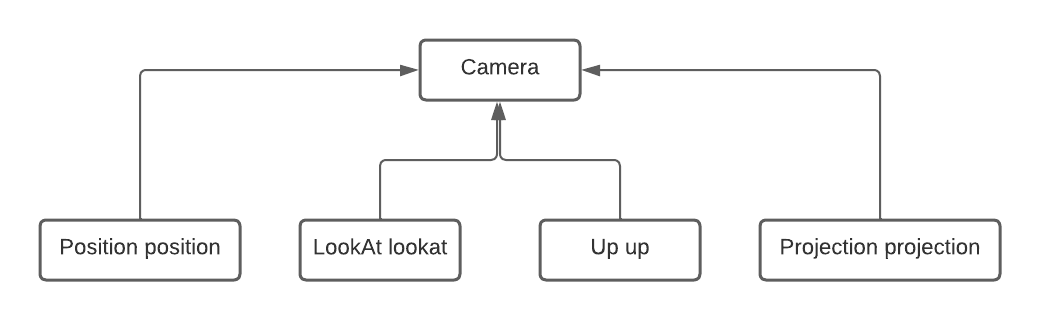
\includegraphics[width=0.8\textwidth]{images/data_structure_camera.png}
	\caption{Estrutura de dados \emph{Camera}} \label{fig:camera}
\end{figure}
\begin{figure}[H]
	\centering
	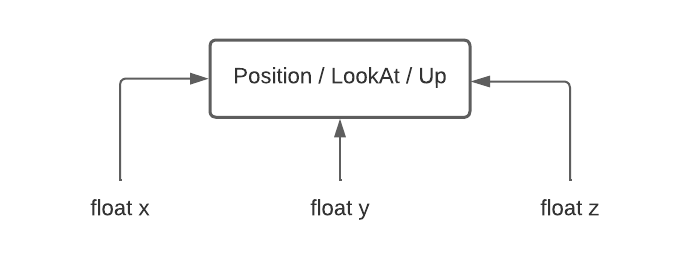
\includegraphics[width=0.6\textwidth]{images/struct_position.png}
	\caption{Estruturas de dados \emph{Position, LookAt e Up}} \label{fig:position}
\end{figure}
\begin{figure}[H]
	\centering
	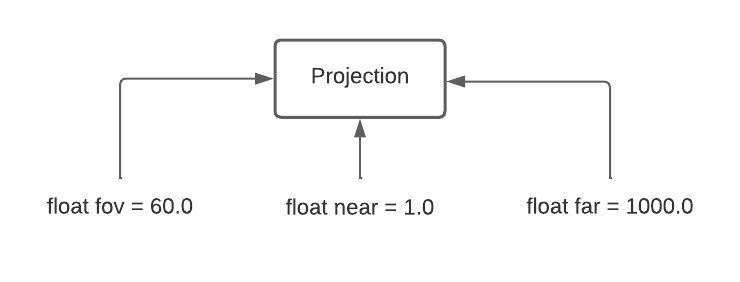
\includegraphics[width=0.6\textwidth]{images/struct_projection.png}
	\caption{Estrutura de dados \emph{Projection}} \label{fig:projection}
\end{figure}
\begin{figure}[H]
	\centering
	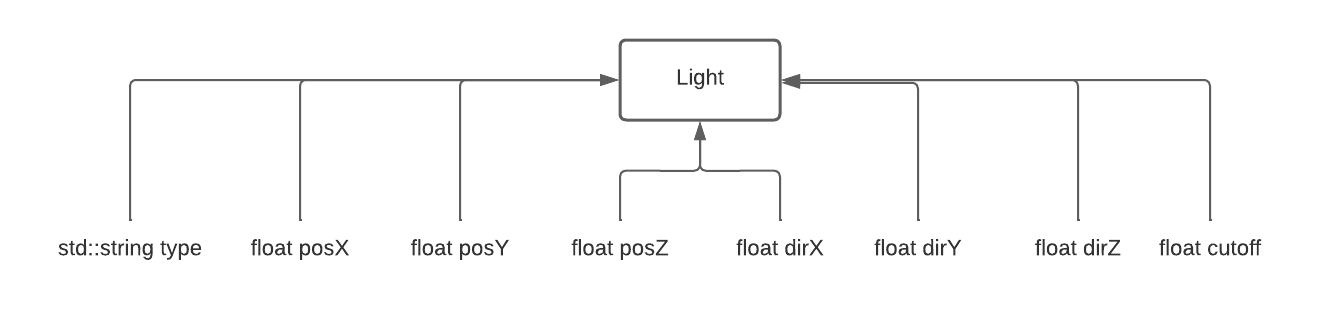
\includegraphics[width=0.9\textwidth]{images/struct_light.png}
	\caption{Estrutura de dados \emph{Light}} \label{fig:light}
\end{figure}
\begin{figure}[H]
	\centering
	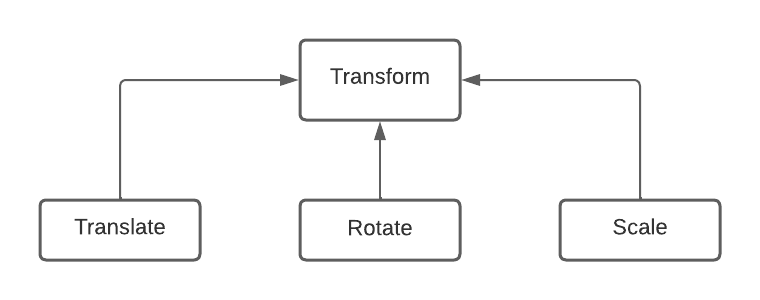
\includegraphics[width=0.6\textwidth]{images/class_transform.png}
	\caption{Classe \emph{Transform}} \label{fig:transform}
\end{figure}
\begin{figure}[H]
	\centering
	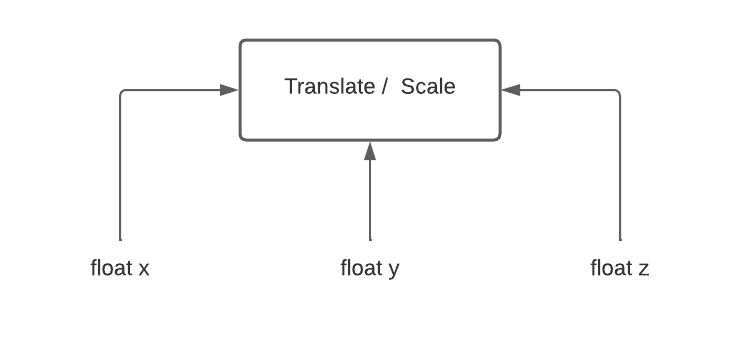
\includegraphics[width=0.6\textwidth]{images/class_translate.png}
	\caption{Classes \emph{Translate} e \emph{Scale}} \label{fig:translate}
\end{figure}
\begin{figure}[H]
	\centering
	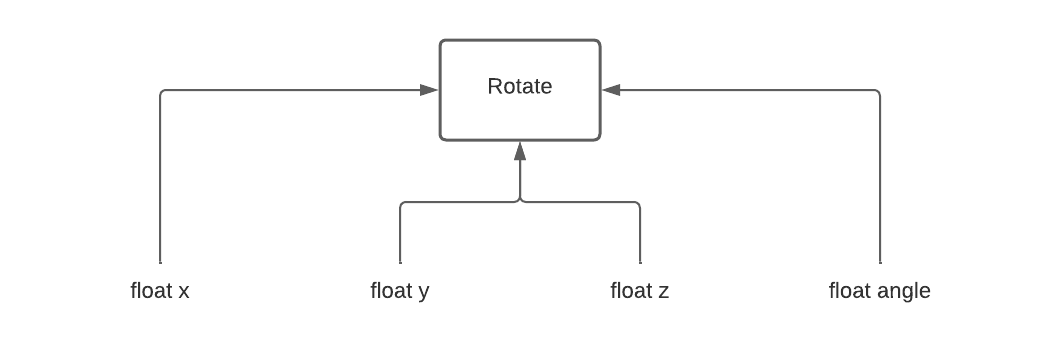
\includegraphics[width=0.8\textwidth]{images/class_rotate.png}
	\caption{Classe \emph{Rotate}} \label{fig:rotate}
\end{figure}
\begin{figure}[H]
	\centering
	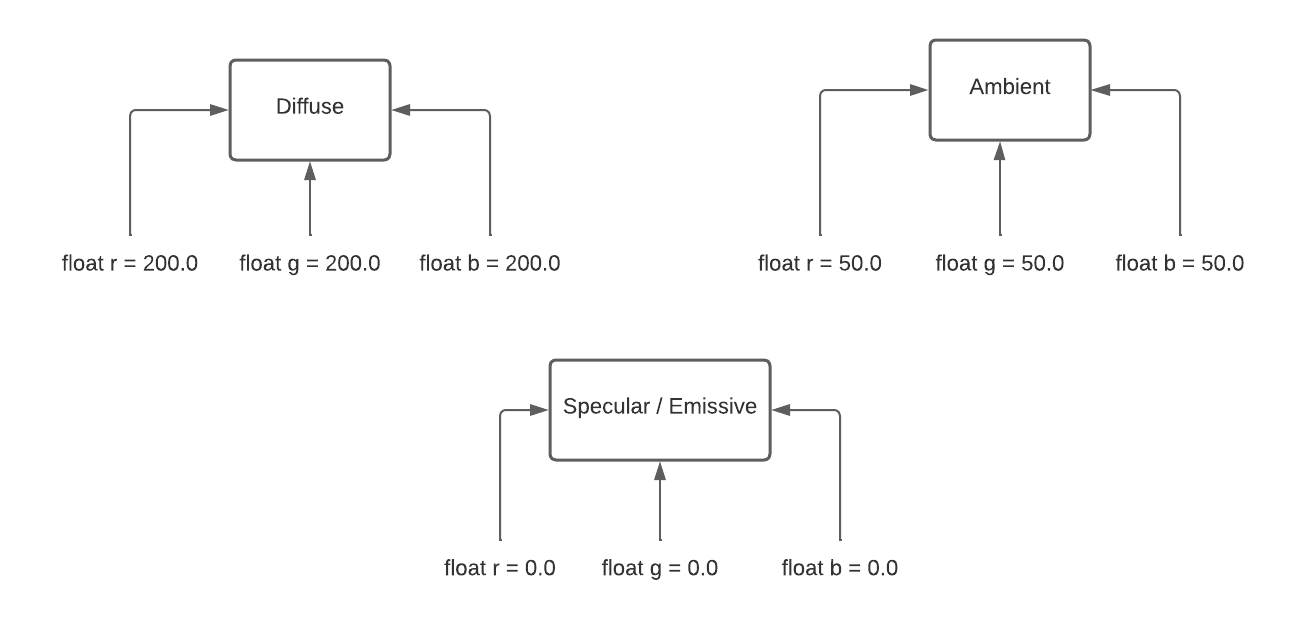
\includegraphics[width=0.8\textwidth]{images/struct_diffuse.png}
	\caption{Estruturas de dados \emph{Diffuse, Ambient, Specular e Emissive}} \label{fig:diffuse}
\end{figure}

As figuras exibidas acima representam as classes e estruturas de dados utilizadas para a estruturação dos dados obtidos na leitura do ficheiro de configuração. De notar que os valores descritos nas figuras indicam os valores padrão das variávies em questão, isto é, os valores que as variáveis tomam quando não especificadas no ficheiro de configuração.

\section{Desenho dos modelos}
No que toca ao desenho dos modelos, desenvolveu-se as seguintes funções:
\begin{itemize}
\item void drawAxis(); \\ Desenha os eixos \emph{x}, \emph{y} e \emph{z};
\item void drawModels(); \\ Desenha os modelos descritos no ficheiro de configuração utilizando a função auxiliar drawFigure;
\item void drawFigure(std::string filename); \\ Desenha os pontos contidos no ficheiro passado como argumento, resultando na figura pretendida. Utiliza a função tokenize como auxiliar;
\item void tokenize(std::string const \&str, const char* delim, std::vector$<$float$>$ \&out); \\ Recebe uma linha com coordenadas, separa-as e coloca-as num vetor, onde a posição 0, 1 e 2 do vetor correspondem às coordenadas x, y e z, respetivamente;
\end{itemize}

\section{Execução do Engine}
O comando utilizado para execução do programa \emph{engine} é: \\ \\
\$: engine $<$configFile.xml$>$ \\ \\ O "configFile.xml" corresponde ao ficheiro de configuração que se pretende utilizar na execução.

\chapter{Concepção/desenho da Resolução}
\section{Estruturas de Dados}
\section{Algoritmos}

\chapter{Testes realizados e Resultados}
\section{Teste nº1}

\begin{lstlisting}[caption={XML do Teste 1}, label={teste1}]
<world> 
    <window width="512" height="512" />
    <camera> 
	    <position x="5" y="-2" z="3" />
	    <lookAt x="0" y="0" z="0" />
	    <up x="0" y="1" z="0" />
        <projection fov="60" near="1" far="1000" /> 
    </camera>
    <group> 
  	<models> 
		<model file="../../3d/cone_1_2_4_3.3d" /> <!-- generator cone 1 2 4 3 cone_1_2_4_3.3d -->
 	</models>
    </group>
</world>
\end{lstlisting}

\begin{figure}[H]
	\centering
	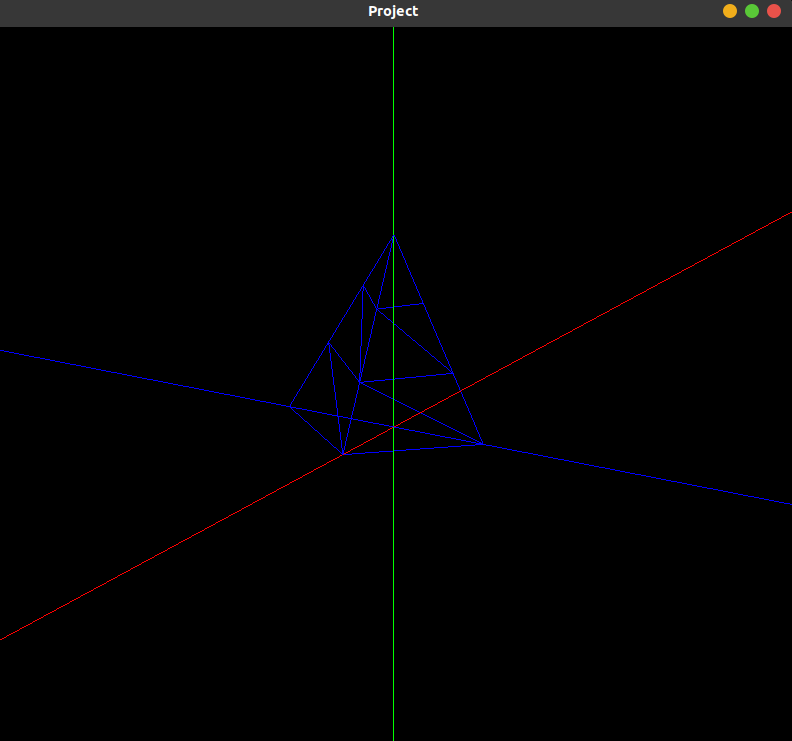
\includegraphics[width=0.7\textwidth]{images/cone.png}
	\caption{Resultado do Teste 1} \label{fig:cone}
\end{figure}

\newpage
\section{Teste nº2}
\begin{lstlisting}[caption={XML do Teste 2}, label={teste2}]
<world> 
    <window width="512" height="512" />
    <camera> 
        <position x="5" y="-2" z="3" />
        <lookAt x="0" y="0" z="0" />
        <up x="0" y="1" z="0" />
        <projection fov="20" near="1" far="1000" /> 
    </camera>
    <group> 
        <models> 
            <model file="../../3d/cone_1_2_4_3.3d" /> <!-- generator cone 1 2 4 3 cone_1_2_4_3.3d -->
        </models>
    </group>
</world>
\end{lstlisting}

\begin{figure}[H]
	\centering
	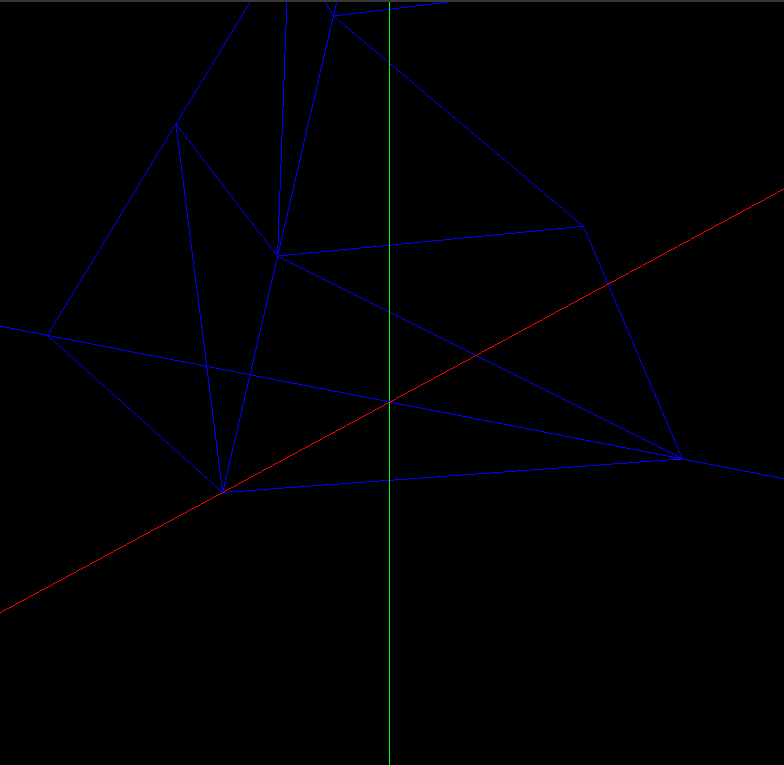
\includegraphics[width=0.7\textwidth]{images/cone2.png}
	\caption{Resultado do Teste 2} \label{fig:cone2}
\end{figure}

\section{Teste nº3}
\begin{lstlisting}[caption={XML do Teste 3}, label={teste3}]
<world> 
    <window width="512" height="512" />
    <camera> 
        <position x="3" y="2" z="1" />
        <lookAt x="0" y="0" z="0" />
        <up x="0" y="1" z="0" />
        <projection fov="60" near="1" far="1000" /> 
    </camera>
    <group> 
        <models> 
            <model file="../../3d/sphere_1_10_10.3d" /> <!-- generator sphere 1 10 10 sphere_1_10_10.3d -->
        </models>
    </group>
</world>
\end{lstlisting}

\begin{figure}[H]
	\centering
	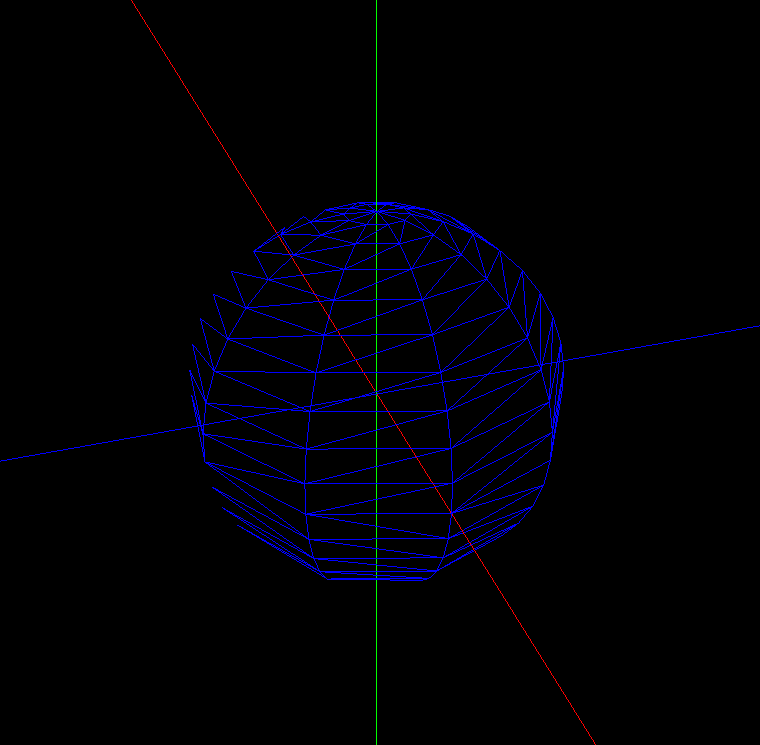
\includegraphics[width=0.7\textwidth]{images/sphere.png}
	\caption{Resultado do Teste 3} \label{fig:sphere}
\end{figure}

\section{Teste nº4}
\begin{lstlisting}[caption={XML do Teste 4}, label={teste4}]
<world> 
    <window width="512" height="512" />
    <camera> 
        <position x="3" y="2" z="1" />
        <lookAt x="0" y="0" z="0" />
        <up x="0" y="1" z="0" />
        <projection fov="60" near="1" far="3.5" /> 
    </camera>
    <group> 
        <models> 
            <model file="../../3d/box_2_3.3d" /> <!-- generator box 2 3 box_2_3.3d -->
        </models>
    </group>
</world>
\end{lstlisting}

\begin{figure}[H]
	\centering
	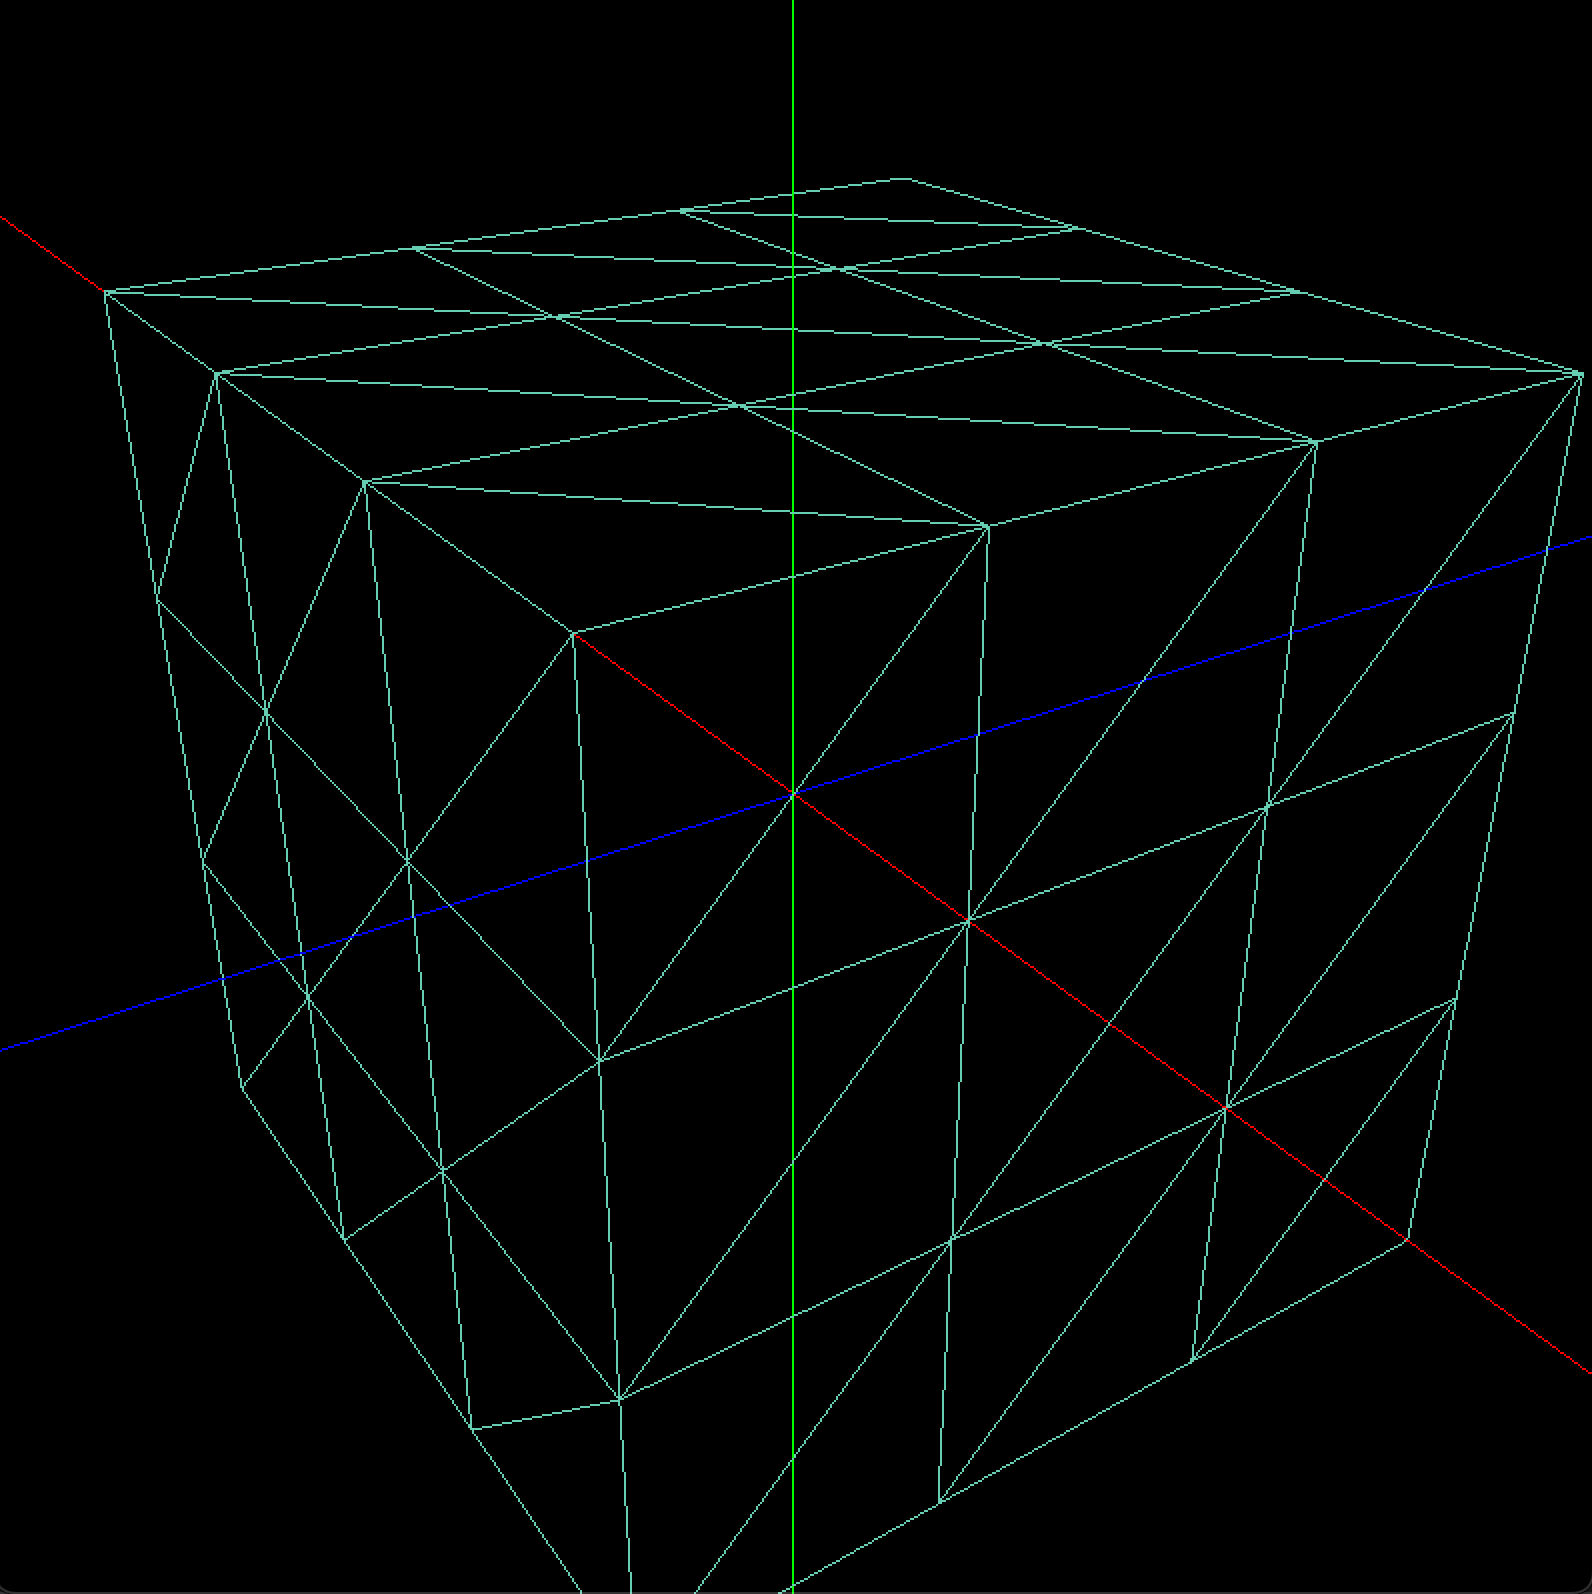
\includegraphics[width=0.7\textwidth]{images/box.png}
	\caption{Resultado do Teste 4} \label{fig:box}
\end{figure}

\section{Teste nº5}
\begin{lstlisting}[caption={XML do Teste 5}, label={teste5}]
<world> 
    <window width="512" height="512" />
    <camera> 
        <position x="3" y="2" z="1" />
        <lookAt x="0" y="0" z="0" />
        <up x="0" y="1" z="0" />
        <projection fov="60" near="1" far="1000" /> 
    </camera>
    <group> 
        <models> 
            <model file="../../3d/plane_2_3.3d" /> <!-- generator plane 2 3 plane_2_3.3d -->
            <model file="../../3d/sphere_1_10_10.3d" /> <!-- generator sphere 1 10 10 sphere_1_10_10.3d -->
        </models>
    </group>
</world>
\end{lstlisting}

\begin{figure}[H]
	\centering
	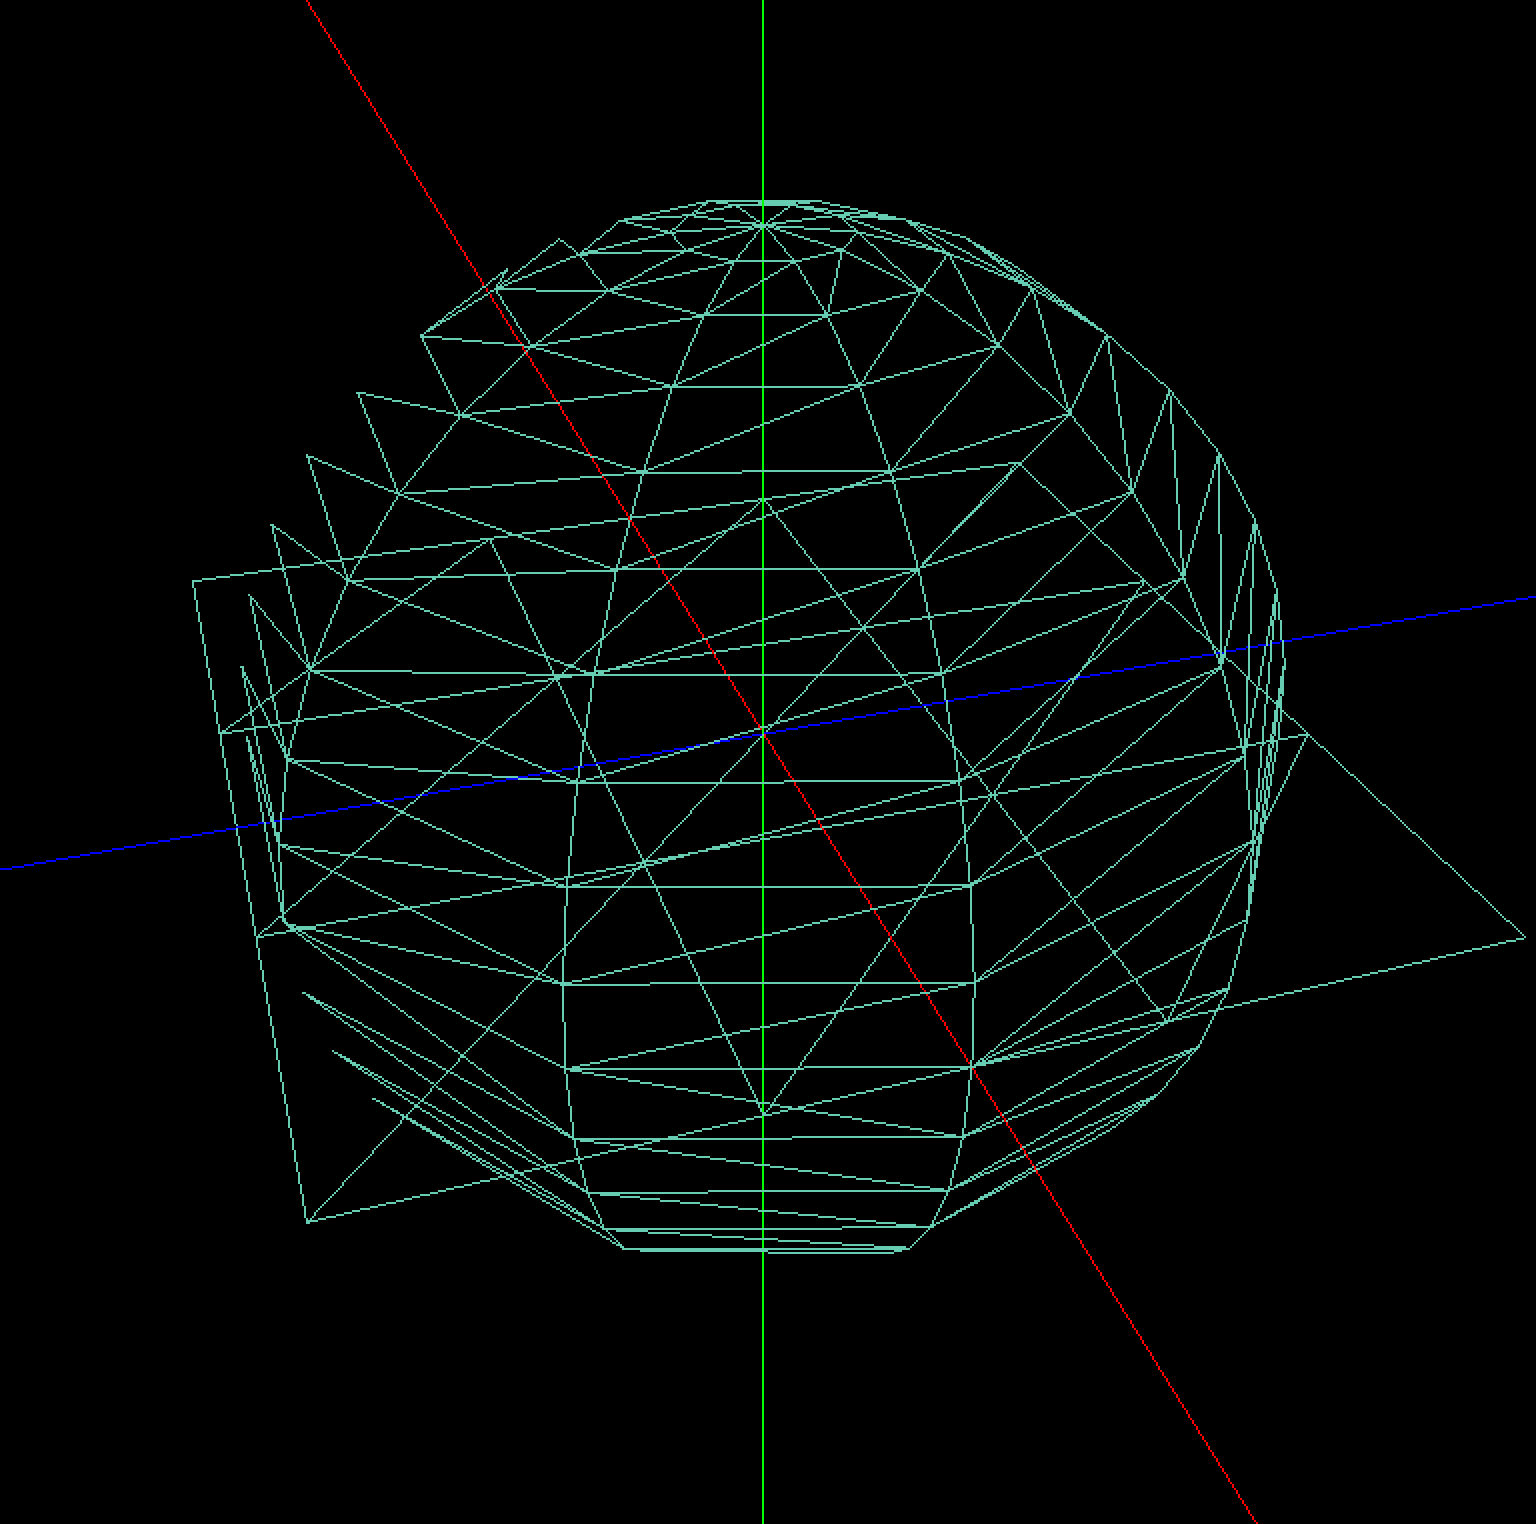
\includegraphics[width=0.7\textwidth]{images/sphere_plane.png}
	\caption{Resultado do Teste 5} \label{fig:sphere_plane}
\end{figure}

%\VerbatimInput{teste1.txt}

\chapter{Conclusão} \label{concl}
Síntese do Documento~\cite{araujo:2018,martini:2018}.\\
Estado final do projecto; Análise crítica dos resultados~\cite{Sto77a}.\\
Trabalho futuro.

\appendix % apendice
\chapter{Código do Programa}

Lista-se a seguir o CÓDIGO \antlr~\cite{antlr:2016} do programa
\darius~\cite{maskin:1985} que foi desenvolvido.
\begin{verbatim}
public class Aula()
  {
    int n, m;
    int max(int a, int b)
      {
       ......
       return(max);
      }
  }
\end{verbatim}

Lista-se a seguir UM TEXTO (COM O COMANDO VERBATIN)
\begin{verbatim}
      aqui deve aparecer o código do programa,
      tal como está formato no ficheiro-fonte "darius.java"
      um pouco de matematica $\$$
      caso indesejável $\varepsilon$
\end{verbatim}


Lista-se a seguir (ver a Listing~\ref{lstExe1} abaixo) UM TEXTO não processado porque fixado COM O COMANDO LISTING 
que embora parecido com o Verbatim é muito mais sofisticado.

\begin{lstlisting}[caption={Exemplo de uma Listagem}, label={lstExe1}]
      ou entao aparecer aqui neste sitio um pouco de matematica $\$$
      como alternativa ao anterior.
      e aqui mais um teste $\varepsilon$
\end{lstlisting}

\newpage


%\lstinputlisting[caption={Exemplo de uma importação}, label={lstExe2}]{listagemImportadaLayout.l} %input de um ficheiro da listagem

%-- Fim do documento -- inserção das referencias bibliográficas

%\bibliographystyle{plain} % [1] Numérico pela ordem de citação ou ordem alfabetica
\bibliographystyle{alpha} % [Hen18] abreviação do apelido e data da publicação
%\bibliographystyle{apalike} % (Araujo, 2018) apelido e data da publicação
                             % --para usar este estilo descomente no inicio o comando \usepackage{apalike}

\bibliography{bibLayout} %input do ficheiro de referencias bibliograficas

\end{document} 